\subsection{Surface Enhanced Raman Spectroscopy with Graphene}

Plasmonics explores the interaction of metallic surfaces and light waves that causes density waves of electrons on the surface. The electron density wave propagating on the metal is often referred to as a surface plasmon. In addition to free plasmons localised surface plasmons are created by exciting a nano structure that is smaller than the wavelength $\lambda$ of the light used for the excitation.

Exciting a localized surface plasmon during Raman processes can increase the intensity of the Raman signal by several orders of magnitude\mcite. This field enhancement is greatest for a resonance between the frequency of the incident light and the frequency of the surface plasmon $\omega_P$. Only the dipolar term of the $\mathbf{E}$ field contributes to the excitation of surface plasmons and therefore in the enhancement of the Raman signal. Because of the influence of the surface plasmons this method is called "Surface Enhanced Raman Spectroscopy".

\begin{figure}[!h]
  \centering
  \begin{subfigure}{0.45\textwidth}
    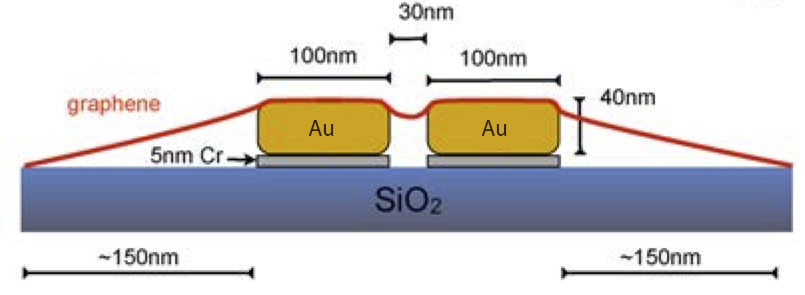
\includegraphics[width=\textwidth]{./images/sers-schema.png}
  \end{subfigure}
  ~
  \begin{subfigure}{0.45\textwidth}
    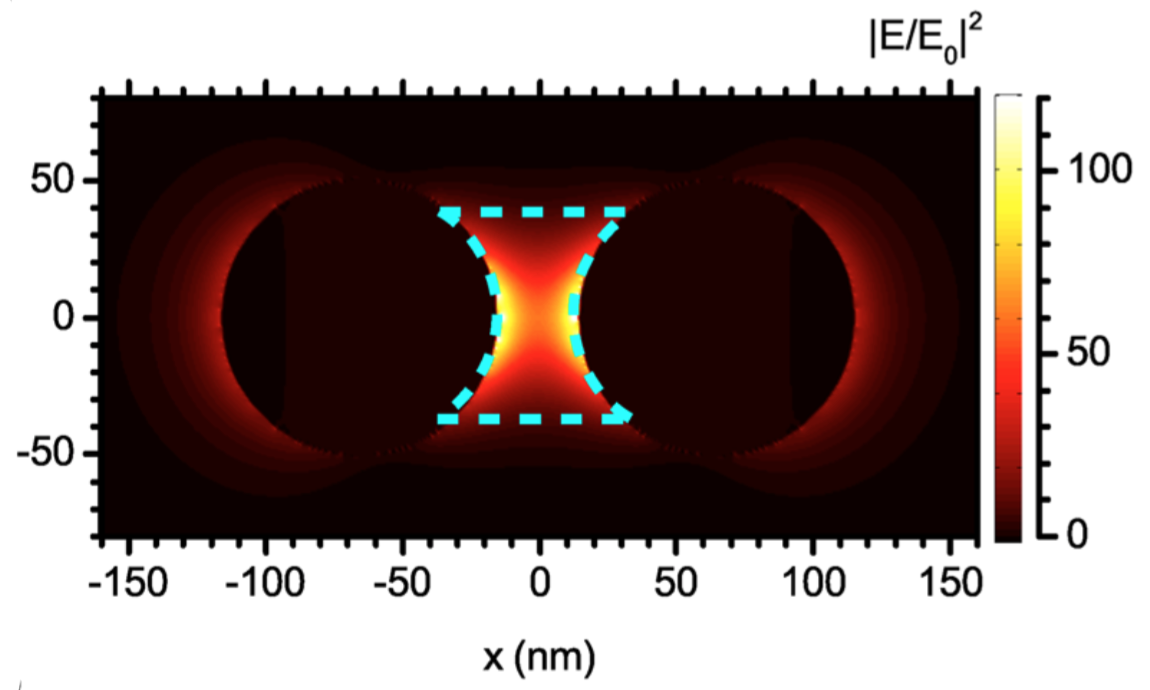
\includegraphics[width=\textwidth]{./images/local-enhancement-heeg.png}
  \end{subfigure}
  \caption{\textbf{(a)} Gold disks are placed with a chrome interlayer on SiO$_2$. A layer of graphene is pulled into the gap. Adapted from \cite{heeg}. \textbf{(b)} Local enhancement at $\lambda = 638nm$ and $z=40nm$. The blue dashed line indicates the area that includes 90\% of the near field intensity according to \cite{heeg}. Copied from \cite{heeg}.}
  \label{fig:heeg-experiment}
\end{figure}

As an example an experiment from \cite{heeg} is shown in figure~\ref{fig:heeg-experiment}. Graphene is put on top of two gold nanostructures with a diameter of \SI{100}{nm} and a distance of \SI{30}{nm}. Localized surface plasmons in the gold structures enhance the Raman signal. The size of the structure is chosen to be in resonance with the laser frequency of $\lambda = 638nm$.

As already noted only the parallel terms of the $\mathbf{E}$-field are contributing to the enhancement which means for graphene that only the component of the electric field that lies within the graphene plane is contributing to the enhancement.

\subsubsection{Electromagnetic Enhancement Theory of SERS}

The effect of the localized surface plasmons actually happens twice: When the incident photons scatter with phonons and excite Raman modes and a second time for the Raman signal. Each enhancement leads to an $|\mathbf{E}|^2/E_0^2$ enhancement, both effects to a total enhancement proportional to $|\mathbf{E}|^4$ as stated in

\begin{equation}
  Enh_{local}(\mathbf{r},\omega_L)=\frac{\left|\mathbf{E}_{loc}(\mathbf{r}, \omega_L)\right|^2}{\left|\mathbf{E}_0\right|^2}\frac{\left|\mathbf{E}_{loc}(\mathbf{r}, \omega_L-\omega_{ph})\right|^2}{\left|\mathbf{E}_0\right|^2}\approx\frac{\left|\mathbf{E}_{loc}(\mathbf{r})\right|^4}{\left|\mathbf{E}_0\right|^4}.
  \label{eq:enhancement}
\end{equation}
